%%%%%%%%%%%%%%%%%%%%%%%%%%%%%%%%%%%%%%%%%%%%%%%%%
%%%%%%%%%%%%%%%%%%%%%%%%%%%%%%%%%%%%%%%%%%%%%%%%%

\chapter{Experimental setup}
\label{chap:experiment}

%%%%%%%%%%%%%%%%%%%%%%%%%%%%%%%%%%%%%%%%%%%%%%%%%
%%%%%%%%%%%%%%%%%%%%%%%%%%%%%%%%%%%%%%%%%%%%%%%%%

This chapter describes the experimental setup for the simulations that were performed for the purposes of this study. Section~\ref{chap:robots} describes the robots used in the study, while the simulation environment is described in Section~\ref{simulator}. The environments used in the experiment are discussed in Section~\ref{experimentenvironments}, and Section~\ref{swarmparameters} defines the parameters for the robot swarm. Section~\ref{experimentation} defines how experiments were performed and performance measures used to evaluate the performance of the algorithms on the prioritized foraging problem are proposed in Section~\ref{thri:third:performancemeasures}. The chapter is summarized in Section~\ref{third:summary}.

%%%%%%%%%%%%%%%%%%%%%%%%%%%%%%%%%%%%%%%%%%%%%%%%%
%%%%%%%%%%%%%%%%%%%%%%%%%%%%%%%%%%%%%%%%%%%%%%%%%

\section{Robots}
\label{chap:robots}

Foraging robots occur in all shapes, sizes and capabilities. Some robots have powerful GPS capabilities and advanced long distance sensors, while others are much simpler. This chapter defines the capabilities of the simulated robots to be used in this study. The robots are described in Section~\ref{robotdescription}, while Section~\ref{navigationandobstacleavoidance} outlines the navigational capabilities of the robots. 

\subsection{Robot Description}
\label{robotdescription}

The artificial robots modelled in this study are based on e-puck robots \cite{mondada2009puck}, with additional grippers. Each simulated robot is equipped with a 360 degree camera to identify objects around the robot, as well as eight local distance sensors equally spaced around the circular perimeter of the robot. Both camera and distance sensors have a depth of view of five times the robot's size. Robots use local communication which can occur in a radius of five times the robot's size. The sensor and communication range is sufficiently localized with respect to the size of the environment. Each simulated robot can forage a single item at a time. The robots do not have a global positioning system (GPS) capability to locate items to position themselves in the environment. A robot can not see occluded items. As a result, the simulated robots have to explore the environment to find the prioritized items.

\subsection{Navigation and Obstacle Avoidance}
\label{navigationandobstacleavoidance}

The environments used in the simulation have a variety of complexities: Some environments are very sparse, while others have large zones of non-prioritized items that must be navigated around or foraged to clear a route to the prioritized items. Due to the environmental complexity, an advanced navigation and obstacle avoidance technique is required.

The robots in the experiments for this thesis use a navigation and obstacle avoidance technique inspired by a congestion avoidance technique developed for communication congestion avoidance in wireless sensor networks \cite{antoniou2012congestion}. Antoniou \textit{et al} use inspiration from the flocking behaviour of birds in order to efficiently route messages around congested areas in wireless sensor networks. In flocking behaviour of birds, birds are attracted by a global magnetic attractor to the birds' final destination, while a local attractor pulls flocking birds away from areas of congestion. In the congestion avoidance algorithm, the final destination of the message being sent on the wireless sensor network is a combination of the global attractor and the local attractor.

The described congestion avoidance technique has been adapted to form a simple but effective navigation and obstacle avoidance technique. Robots are pulled to a global attractor, which is the intended destination, while a local attractor directs robots away from local obstacles while maintaining a course to the destination.

Figure \ref{fig:obstacleavoidance} illustrates the navigation and obstacle avoidance method used by the robots. The navigation and obstacle avoidance algorithm achieves the effect of the global attractor by setting the robots' field of view towards the direction of the desired destination. The destination is determined by a homing beacon or by the robot's path integration vector. The direction at the centre of the field of view is the direction to the destination. 

\begin{figure}
	\centering
	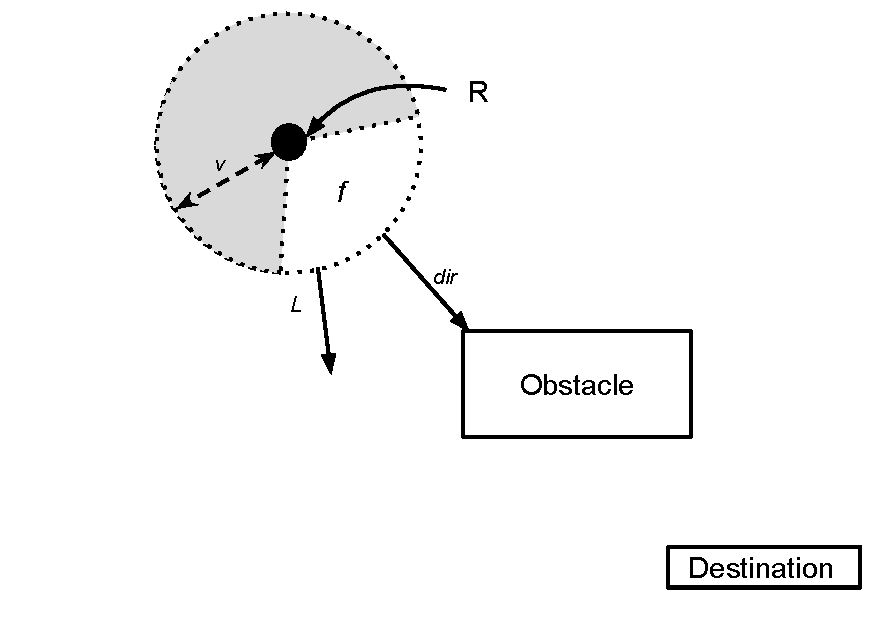
\includegraphics[width=0.75\textwidth]{chapters/chapter5/figures/ObstacleAvoidance.pdf}
	\caption{Navigation and obstacle avoidance, where $v$ is depth of view, $f$ is the field of view, $R$ is the robot, $dir$ is the direction of the destination and $L$ is a possible value of local attractor}
	\label{fig:obstacleavoidance}
\end{figure}

The effect of the local attractor is modelled by evaluating each direction in the field of view to select the most desirable direction. Desirability, $d$, of a direction, $q$, is a metric quantifying the how well a direction achieves a balance between clarity of the path and directness of the direction to the destination. The clarity, $\kappa_q$, in a direction $q$, is a normalized reading from the proximity sensor or camera such that $\kappa_q\in[0,1]$. Clarity indicates the distance to the next nearest obstacle. If no obstacles exist in the depth of view $v$, then  $\kappa_q=0$. If there exists an obstacle immediately next to the robot, then $\kappa_q=1$. The directness of a direction $q$, $\iota_q\in[0,1]$ is calculated as the angular deviation from the direction of the destination, where $\iota_q=0$ occurs when the direction $i$ is the same as direction to the destination, $dir$, and a $\iota_q=1$ occurs when the direction is at the edge of the field of view, $f$. Desirability $d_q$ of direction $q$ is defined as

\begin{equation}
	d_i= \lambda \kappa_q + (1 - \lambda)\iota_q \\
	\label{eq:1}
\end{equation} where $\lambda$ determines whether clarity, $\kappa_q$, or directness, $\iota_q$, of direction $q$, has a greater effect on desirability. The described navigation and obstacle avoidance technique is used with all algorithms in the experiment and for all algorithms, $\lambda$ is set to 0.5.




%%%%%%%%%%%%%%%%%%%%%%%%%%%%%%%%%%%%%%%%%%%%%%%%%
%%%%%%%%%%%%%%%%%%%%%%%%%%%%%%%%%%%%%%%%%%%%%%%%%
\section{Simulator}
\label{simulator}
A spatially discrete 2-dimensional grid world simulator has been developed and used in this thesis in order to accelerate computation. Discrete 2-dimensional grid world simulators are also used in \cite{sugawara2002swarming, hecker2015beyond}. In real robot experiments, algorithm performance is sensitive to the amount of time taken to load items and manoeuvre the robots \cite{ostergaard2001emergent}. The 2-dimensional grid world simulator allows for movement and loading time to be standardized across all algorithms for effective comparison.

The simulated robots function as follows:
\begin{itemize}
	\item Each robot fits into one grid block and each item takes up one grid block. 
	\item Only a single object can occupy a grid block at a time.  An object is either a robot or an item. Since only one object can occupy a grid block at a time, collisions and congestion can occur.
	\item Each robot can move to an adjacent cell in any direction.
	\item Robots can load, transport and offload a single item at a time.
	\item If a robot cannot pick up an item, the item is an obstacle that a robot may have to navigate around in order to reach its destination.
\end{itemize}

The prioritized and non-prioritized sinks were placed next to each other, on a single side of the environment. The sinks were marked by beacons that all robots can detect and navigate towards. The reason why the sinks were not placed in the centre of the environment, as is commonly found in swarm robotics research \cite{labella2006division}, is because the prioritized foraging problem is inspired from using a swarm of robots to rescue trapped miners in mining tunnels, discussed in Section~\ref{sec:second:prioritizedforaging}. A mining tunnel has a single entrance where the gold and waste must be moved to, in order to be transported to the surface \cite{brune2010extracting}. Since there is only a single entrance at the beginning of a tunnel, the sinks need to occur at the beginning of the tunnel so that items can be easily exported.

\section{Environments}
\label{experimentenvironments}

In order to test flexiblity on different environment types, many types of environments should be examined. This section defines the various environments and presents how they were generated. Section~\ref{environmentalparameters} discusses the parameters for the environments, while different environment distributions, and the algorithms to generate those distributions are presented in Section~\ref{environmentdistributions}. Finally, the accessible environment is defined in Section~\ref{accessibleenvironment}.

\subsection{Environmental Parameters}
\label{environmentalparameters}
The experiments were run on different environments where each environment has different item distributions, environment sizes, item densities, and different ratios of prioritized to non--prioritized items. All the environments are square. The length and width of the square environment grid is denoted as $\Lambda$, where $\Lambda\in \left\{ 50, 100, 200, 300, 500\right\}$.

Different values for the density, $p$, of the items on the grid were chosen, such that if $p=0.9$, then 90\% of the grid cells are occupied by items, where $p\in \{ 0.05,\allowbreak 0.2,\allowbreak 0.5,\allowbreak 0.7,\allowbreak 0.9\}$. Environments with a larger item density are more complex to forage, because there exists a higher probability that items will occlude each other. Thus, a robot may not be able to access items of the type that it is specialized to forage, since its access to those items is occluded by items of a different type. For this reason, we refer to the density of items on the grid as the problem complexity.

The environment type ratio, $r$, is defined as the ratio of prioritized to non-prioritized items in an environment, where $r\in \{0,\allowbreak 0.2,\allowbreak 0.25,\allowbreak 0.33,\allowbreak 0.5,\allowbreak 0.67,\allowbreak 0.75,\allowbreak 0.8, 1\}$. When $r=0$, an environment contains no prioritized items, and when $r=1$, only prioritized items exist in the environment. Environments with a small $r$ value have an abundance of non-prioritized items which increases the likelihood of non-prioritized items preventing access to prioritized items.

\subsection{Environment Distributions}
\label{environmentdistributions}
The environment distribution, $\epsilon$, is defined as the distribution of prioritized and non-prioritized items in an environment, such that $\epsilon\in\{uniform, clustered, gaussian, vein\}$. Each environment distribution was chosen in order to examine different characteristics of the algorithms. The item distributions are illustrated in Figure~\ref{fig:environments}, where each lighter shaded square is a prioritized item and a non-prioritized item is shown by a darker shaded square. The four environment distributions were generated as follows:

\begin{figure} [h]
        \centering
        \begin{subfigure}[b]{0.21\textwidth}
                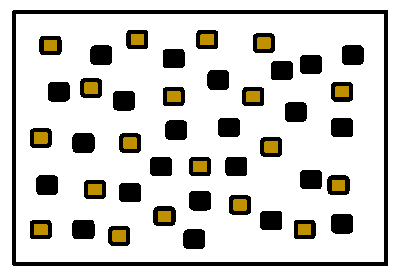
\includegraphics[width=\textwidth]{chapters/chapter4/figures/uniformenv.pdf}
                \caption{Uniform}
                \label{fig:uniformenv}
        \end{subfigure}%
		\begin{subfigure}[b]{0.2\textwidth}
                        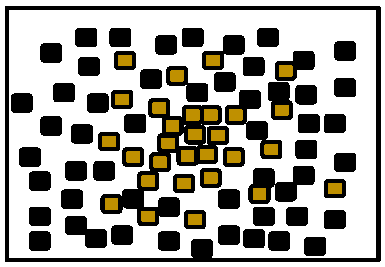
\includegraphics[width=\textwidth]{chapters/chapter4/figures/gaussianenv}
                        \caption{Gaussian}
                        \label{fig:gaussianenv}
       \end{subfigure}
        \begin{subfigure}[b]{0.205\textwidth}
                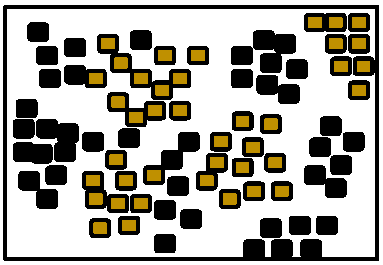
\includegraphics[width=\textwidth]{chapters/chapter4/figures/clusterenv.pdf}
                \caption{Clustered}
                \label{fig:clusterenv}
        \end{subfigure}
        \begin{subfigure}[b]{0.2\textwidth}
                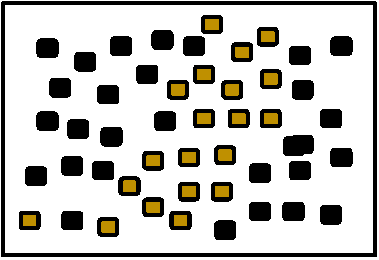
\includegraphics[width=\textwidth]{chapters/chapter4/figures/veinenv.pdf}
                \caption{Vein}
                \label{fig:veinenv}
        \end{subfigure}  

		\caption{Environment Classes}
		\label{fig:environments}
\end{figure}

\begin{algorithm}

\caption{Uniform Distributed Environments}
\label{algorithm:uniform}
\begin{algorithmic}[1]
\Function{uniform}{$numberItems, r, S$}
	\State \text{nonPrioritizedItemsLeft = floor((1-$r$)*numberItems)}
	\State \text{prioritizedItemsLeft = floor( $r$*numberItems)}
	\While{\text{$prioritizedItemsLeft > 0$}}
		\State \text{x $\gets$ uniform(0, S)}
		\State \text{y $\gets$ uniform(0, S)}
		\If{\text{gridCell (x,y) is empty}}
			\State \text{Place prioritized item at (x,y)}
			\State \text{Decrement $prioritizedItemsLeft$}
		\EndIf
	\EndWhile

	\While{\text{$nonPrioritizedItemsLeft > 0$}}
		\State \text{x $\gets$ uniform(0, S)}
		\State \text{y $\gets$ uniform(0, S)}
		\If{\text{gridCell (x,y) is empty}}
			\State \text{Place prioritized item at (x,y)}
			\State \text{Decrement $nonPrioritizedItemsLeft$}
		\EndIf
	\EndWhile
\EndFunction
\end{algorithmic}
\end{algorithm}

\begin{enumerate}

\item The position of each item in a uniformly distributed environment is selected from a uniform distribution (refer to Figure~\ref{fig:uniformenv}). The uniformly distributed environment has uniform concentrations of prioritized and non-prioritized items across the environment and thus is used as a control environment. Pseudo-code for generation of uniform environments is provided in Algorithm~\ref{algorithm:uniform}.

\item For the Gaussian environments, the positions of the prioritized items are sampled from a Gaussian distribution. The mean of the Gaussian disitribution is the centre of the grid. The deviation of the Gaussian distribution was selected as $deviation = S*E_p/2$ to ensure that generation took a reasonable amount of time (that the same positions are not reselected regularly), and that the non-prioritized items are densely concentrated  (refer to Figure~\ref{fig:gaussianenv}). Pseudo-code for generation of Gaussian environments is provided in Algorithm~\ref{algorithm:gaussian}. The positions of the non-prioritized items are selected from a uniform distribution, after placing the prioritized items. 

In Gaussian distributed environments, prioritized items  occur in high concentration towards the center of the environment. More non-prioritized items occur on the outskirts of the environment, surrounding the prioritized items in the centre.

The Gaussian environments are used to examine whether each algorithm will enable the robot swarm to forage or navigate past the non-prioritized items to reach the high concentration of prioritized items in the environment's centre. 


\item Environments with a vein distribution resemble the patterns observed in naturally occurring gold reefs \cite{frimmel2002recent} (refer to Figure~\ref{fig:veinenv}). In a gold reef, molten gold fills planar fractures between rock resulting in a vein of gold. Inspired by gold reefs, vein distributed environments have a long thin vein of prioritized items running from one side of the environment to another. The vein of prioritized items was surrounded by non-prioritized items. 

The vein environments aimed to test whether a swarm of robots could forage the continuous length of the vein of prioritized items, before foraging non-prioritized items. A swarm that is able to detect the location of the vein and return to the vein's location after foraging an item should forage more prioritized items initially than an algorithm that cannot detect and remember the location of the vein.  Pseudo-code for generation of vein environments is provided in Algorithm~\ref{algorithm:vein}.


\item Environments with a clustered item distribution have a random number of clusters of items of the same type (refer to Figure~\ref{fig:clusterenv}). After clusters have been generated, each cluster is labelled randomly (with a Bernoulli disitribution with probability equal to the item ratio, $r$, required for that environment), as either a cluster of prioritized items or a cluster of non-prioritized items.

The goal of performing experiments in a clustered environment was to test an algorithm's ability to exploit areas which are rich in prioritized items. Clustered environments are also used to test whether an algorithm can either navigate around or forage non-prioritized items. A clustered environment can also test an algorithm's ability to remember locations of areas which have a high density of prioritized items in order to aid more efficient access to prioritized items.  Pseudo-code for generation of clustered environments is provided in Algorithm~\ref{algorithm:clustered} and Algorithm~\ref{algorithm:clustered2}.


\end{enumerate} 

To summarize, the challenges introduced by the more complex distributions (the Gaussian, clustered and vein environment) aim to test a swarm's ability to:

\begin{itemize}
\item navigate past obstacles efficiently, or alternatively, to forage obstacles efficiently, and to
\item return to areas rich in prioritized items to forage these areas.
\end{itemize}



\begin{algorithm}
\caption{Gaussian Distributed Environments}
\label{algorithm:gaussian}
\begin{algorithmic}[1]
\Function{gaussian}{$numberItems, r, S$}
	\State \text{Calculate environment centre point $(x_c, y_c)$}
	\State \text{prioritizedItemsLeft = floor($r$*numberItems)}
	\State \text{nonPrioritizedItemsLeft = floor((1-$r$)*numberItems)}
	\State \text{deviation = S*$r$/2}
	\While{\text{$prioritizedItemsLeft > 0$}}
		\State \text{$x \gets floor(gaussian(x_c, deviation))$}
		\State \text{$y \gets floor(gaussian(y_c, deviation))$}
		\If{\text{gridCell (x,y) is empty and is valid}}
			\State \text{Place prioritized item at (x,y)}
			\State \text{Decrement $prioritizedItemsLeft$}
		\EndIf
	\EndWhile

	\While{\text{$nonPrioritizedItemsLeft > 0$}}
		\State \text{x $\gets$ uniform(0, S)}
		\State \text{y $\gets$ uniform(0, S)}
		\If{\text{gridCell (x,y) is empty}}
			\State \text{Place non prioritized item at (x,y)}
			\State \text{Decrement $nonPrioritizedItemsLeft$}
		\EndIf
	\EndWhile
\EndFunction
\end{algorithmic}
\end{algorithm}


\begin{algorithm}
\caption{Vein Distributed Environments}
\label{algorithm:vein}
\begin{algorithmic}[1]
\Function{vein}{$numberItems, r, S$}
	\State \text{Select two random sides from the grid}
	\State \text{Select a random points on each sides, $(x_0,y_0)$ and $(x_1,y_1)$}
	\State \text{Calculate gradient of vein, $m = (y_0 - y_1)/(x_0 - x_1)$}
	\State \text{Calculate $c$ of equation for line vein, $c = (y_0 - m*x_0)$
}

	\State \text{prioritizedItemsLeft = floor($r$*numberItems)}
	\State \text{nonPrioritizedItemsLeft = floor((1-$r$)*numberItems)}

	\While{\text{$prioritizedItemsLeft > 0$}}
		\State \text{$x \gets uniform(min(x_0,x_1), max(x_0, x_1))$}
		\State \text{$y \gets m*x + c$}
		\If{\text{gridCell (x,y) is valid and gridCell (x,y) is empty}}
			\State \text{Place prioritized item at (x,y)}
			\State \text{Decrement $prioritizedItemsLeft$}
		\EndIf
	\EndWhile

	\While{\text{$nonPrioritizedItemsLeft > 0$}}
		\State \text{x $\gets$ uniform(0, S)}
		\State \text{y $\gets$ uniform(0, S)}
		\If{\text{gridCell (x,y) is empty}}
			\State \text{Place nonprioritized item at (x,y)}
			\State \text{Decrement $nonPrioritizedItemsLeft$}
		\EndIf
	\EndWhile
\EndFunction
\end{algorithmic}
\end{algorithm}


\begin{algorithm}

%TODO
\caption{Clustered Distributed Environments (Part 1)}
\label{algorithm:clustered}
\begin{algorithmic}[1]
\Function{clustered}{$numitems, r, S$}
  \State \text{Generate number of clusters, $total = uniform(3,15)$}
  \State \text{Calculate number of prioritized clusters, $clusters_p = floor(r*total)$}    
  \State \text{Calculate number of non-prioritized clusters, $clusters_{np} = floor((1-r)*total)$}
  
  \State \text{Calculate number of prioritized items, $total_p = floor(r*numitems)$}
  
  \State \text{Calculate number of non-prioritized items, $total_{np} = floor((1-r)*numitems)$}
  
  \State \text{$ave_p = total_p/clusters_{p}$}
  \State \text{$ave_np = total_{np}/clusters_{np}$}
  \State \text{$clustersToGenerate_p = clusters_p$}
  \State \text{$clustersToGenerate_{np} = clusters_{np}$}

  \While{\text{$clustersToGenerate_p > 0$}}
    \State \text{sample centroid for cluster $C$ (x,y) uniformly from grid}
    \State \text{$num_p = uniform(ave_p/2$, $2*ave_p$)}
    \State \text{Calculus radius, $r$, of cluster $C$ as $r = \sqrt{num_p/\pi}$}
    \If{\text{cluster $C$ does not collide with existing clusters}}
      \State \text{Save centroid and radius of cluster $C$ to list}
      \State \text{Decrement $clustersToGenerate_p$}
      \State \text{$itemsToGenerate_p = num_p$}
          
      \While {$itemsToGenerate_p > 0$}
        \State \text{$x_p = gaussian(x, r)$}
        \State \text{$y_p = gaussian(y, r)$}
        \If{\text{position $(x_{p},y_{p})$ is valid}}
          \State \text{Place prioritized item at $(x_p,y_p)$}
          \State \text{Decrement $itemsToGenerate_{np}$}	
        \EndIf
      \EndWhile
    \EndIf
  \EndWhile
  \algstore{clusteredalg}
\end{algorithmic}
\end{algorithm}
  
\begin{algorithm}

%TODO
\caption{Clustered Distributed Environments (Part 2)}
\label{algorithm:clustered2}
\begin{algorithmic}[1]
  \algrestore{clusteredalg}
  \While{\text{$clustersToGenerate_{np} > 0$}}
	  \State \text{sample centroid for cluster $C$ (x,y) uniformly from grid}
	  \State \text{$num_{np}=uniform(ave_{np}/2,2ave_{np})$}
	  \State \text{Calculus radius, $r$, of cluster $C$ as $r = \sqrt{num_{np}/\pi}$}
	  \If{\text{cluster $C$ does not collide with existing clusters}}
	
		  \State \text{Save centroid and radius of cluster $C$ to list}
		  \State \text{Decrement $clustersToGenerate_{np}$}
		  \State \text{$itemsToGenerate_{np} = num_{np}$}
				
		  \While {$itemsToGenerate_{np} > 0$}
        	\State \text{$x_p = gaussian(x, deviation=r)$}
        	\State \text{$y_p = gaussian(y, deviation=r)$}
			\If{\text{position $(x_{np},y_{np})$ is valid}}
				  \State \text{Place non-prioritized item at $(x_{np},y_{np})$}
				  \State \text{Decrement $itemsToGenerate_{np}$}	
			  \EndIf
		  \EndWhile
		\EndIf
	\EndWhile
\EndFunction
\end{algorithmic}
\end{algorithm}


\subsection{Accessible Environment}
\label{accessibleenvironment}

To aid discussions about the algorithms' performance on different types of environments, the concept of an \textbf{accessible environment} should be introduced. For the purposes of this thesis, an accessible environment is the parts of the environment that can be foraged by the swarm and are not blocked by other items. Items that are hidden behind other items are not accessible to the robot swarm and are thus not part of the accessible environment. The accessible environment is much larger in a less densely populated environment. This also introduces the concept of the environment ratio of a given accessible environment. For example, an environment may have a high ratio of prioritized items overall, but if the prioritized items are surrounded completely by non-prioritized items, then the accessible environment consists only of non-prioritized items and has an environmental item type ratio of 0. The environment ratio of the accessible environment changes differently per environment disitribution type. In high density Gaussian environments, the accessible environment will initially consist of mostly non-prioritized items, but as robots forage towards the centre, the accessible environment will consist largely of prioritized items. For uniform environments, all accessible environments would have a similar or same environment item ratio as the entire environment. In clustered environments, depending on the configuration of the clusters, the environment ratio of the accessible environments would vary. For vein environments, at the beginning of foraging, the accessible environment ratio would be low in high density environments if the vein is perpendicular to the sink since only the ``entrance" of the prioritized vein would be exposed to the robots and the rest of the prioritized items would be stacked behind those items. 

\section{Swarm parameters}
\label{swarmparameters}

For all algorithms, each robot swarm was initialized with a swarm specialization ratio, $\tau\in\left\{0, 0.2, 0.25, 0.333, 0.5, 0.667, 0.75, 0.8,1\right\}$. The swarm specialization ratio is the ratio of robots foraging prioritized items to non-prioritized items. When no robots are set to initially forage prioritized items, then $\tau=0$ and when all robots are set to initially forage prioritized items, then $\tau=1$.

The ability of an algorithm to adapt the value of $\tau$ appropriately for a given $r$ indicates the flexibility of the algorithm.

The swarm density, $c$, is defined as the number of cells occupied by a robot, as a percentage of the grid size $\Lambda$ (the length of the side of an environment), where values of $c\in\left\{0.1, 0.3, 0.5, 0.7, 1\right\}$ were evaluated. The swarm density is varied in order to test the scalability of the algorithm. The swarm density is also varied to test each algorithms' ability to adjust the number of actively foraging robots to the density of the items in the environment, $c$, as well as to adjust the number of robots actively foraging an item type, $\tau$, to the item type density, $r$.

The honey bee algorithm specific parameters were selected based on \cite{seeley2009wisdom}, where $t_{wait}=200$ time steps, $f_{max}=100$ time steps, $\Phi=0.8$ and $\rho=0.1$. Testing the effect of each of the parameters specific to the honey bee algorithm was not in the scope of this thesis.

\section{Experimentation}
\label{experimentation}

The initial position of each robot was randomly selected, adjacent to the sink. For the na\"ive algorithm and desert ant algorithm, all robots began in the exploration state. For the honey bee algorithm, all unemployed foraging robots were initialized in the waiting state, and the scout robots were initialized in the explore state. 
An experiment is defined as the 30 independant runs for each algorithm, with a specific set of swarm parameters, and on an environment which has a specific set of environmental parameters. An experiment is run for every possible combination of swarm and environmental parameters.

\section{Performance measures}
\label{thri:third:performancemeasures}

The performance of swarm robotics algorithms can be measured by examining the algorithm's ability to perform a task in terms of efficiency, scalability, flexibility, and robustness.

\subsection{Foraging Efficiency}
\label{setup:foragingefficiency}
The foraging efficiency, $E_P$, of an algorithm is defined as the ratio of the number of prioritized items collected by all robots in a fixed time period on a specific environment to the total number of prioritized items that exist in the environment. The foraging efficiency metric is similar to the efficiency metric used by Hecker \textit{et al} \cite{hecker2015beyond}. The metrics used in experiments performed by Hecker \textit{et al} evaluate the performance of foraging algorithms and are thus appropriate for use in the experiments of this study. The foraging efficiency measure, $E_P$, only considers the prioritized items for the prioritized foraging problem.


\subsection{Flexibility}
\label{setup:flexibility}

As stated in Section~\ref{flexibility}, flexibility refers to the effect of variations in the environment and tasks on the co-ordination mechanisms of swarm robotics algorithms. An algorithm that is highly flexible is one that has been optimized for a specific environment, but is equally efficient on a different environment \cite{hecker2015beyond}.

The flexibility performance measures used in this study are based on the flexibility performance measures used in \cite{hecker2015beyond}, which have been adapted for the prioritized foraging problem by only taking into account the prioritized item. The flexibility study addresses two aspects: Flexibility with respect to different prioritized item ratios, $r$, and flexibility with respect to different environment distributions.

\subsubsection{Notation}

In order to more succinctly define the flexibility performance measures, the following notation is defined:

Let $\overline{r}$ be the list containing all considered elements for environment item type ratio, $r$, and let $n_r$ be the number of elements in the list. Let $\overline{\tau}$ be the list containing all considered elements for initial swarm specialization ratio, $\tau(0)$, and let the number of elements in the list be $n_t$. Similarly, let $\overline{\epsilon}$ be a list of each environment distribution and let $n_\epsilon$ be the number of elements in the list.

Let $Z$ be a matrix of dimensions $n_t \times n_r$. Define each entry of the matrix $Z_{ij}$ as the average foraging efficiency, $E_P$, over all experiments, for a specific environment ratio $r_j$, where $r_j$ is the $j$th element of $\overline{r}$, and for a specific initial swarm specialization ratio $\tau_i(0)$, such that $\tau_i(0)$ is the $i$th element of $\overline{\tau}$.

Similarly, define matrix $D$ with dimensions $n_t \times n_\epsilon$, such that each entry of the matrix $D_{ij}$ is the average foraging efficiency, over all experiments with environment distribution, $\epsilon_j$, and with the initial swarm initialization ratio, $\tau_i(0)$.


\subsubsection{Flexibility with respect to different prioritized item ratios}
\label{setup:flexibility:prioritizeditemratio}

The goal of examining flexibility over different prioritized item ratios is to determine how well the optimum value for initial swarm specialization ratio, $\tau(0)$, for a specific environment item ratio, $r_u$, generalizes across all other environment item ratios, $r_v$, where $u,v = 1,...,n_r$ and $u \neq v$. The optimum value for $\tau(0)$ for environments of a specific environment item ratio is the value that yields the greatest average efficiency for those environments.

To do so, a list $I$ of size $n_r$ is defined, where each entry $I_j$ is set to the index $k$ that yields the maximum value for $Z_{ij}$, for $i = 1,..., n_\tau$, for environments with a specific environment type ratio $r_j$. More succinctly:

\begin{equation}
I_j = ( k | Z_{kj} = \max_{i=1,...,n_\tau}\{Z_{ij}\} )
\end{equation}

The moment, $F_{r_u}$, around the maximum foraging efficiency for a specific environment item type ratio, $r_u$, is defined as follows: 

\begin{equation}
F_{r_u} = \sum_{v=1}^{n_r}\dfrac{|Z_{I_uu}- Z_{I_uv}|}{Z_{I_uu}}
\end{equation}

The final performance measure is the normalized sum of the above moments around the maximum foraging efficiency for every environment item type ratio in $\overline{r}$:

\begin{equation}
F_r = \dfrac{1}{n_r}\sum_{u=1}^{n_r} F_{r_u}
\end{equation}

The performance measure, $F_r$, measures how well swarm parameters, which are optimized to yield the best efficiency for environments with a specific prioritized item ratio generalize across environments with different prioritized item ratios. The less the foraging efficiency varies when an algorithm that is configured with swarm parameters optimized for a specific environment ratio, is run on all other environment ratios, the smaller $F_r$ will be. Therefore, the smaller $F_r$ is, the more flexible an algorithm is considered to be. $F_r$ is a macro performance indicator which is run on the results of all experiments. 


\subsubsection{Flexibility with respect to different environment distributions}
\label{setup:flexibility:environmentdistributions}


This performance measure evaluates flexibility by analysing how well swarm parameters, which are optimized to yield the best efficiency for environments with a specific environment distribution generalize across environments with different environment distributions. The performance measure, $F_{\epsilon}$, is defined similar to $F_r$, except over environment distributions, rather than environmental item ratios. A list $Y$ of size $n_\epsilon$ is defined as follows:

\begin{equation}
Y_j = ( k | D_{kj} = \max_{i=1,...,n_\tau}\{D_{ij}\} )
\end{equation}

The performance measure, $F_\epsilon$, is defined as follows:

\begin{equation}
F_\epsilon = \dfrac{1}{n_\epsilon}\sum_{u=1}^{n_\epsilon} \sum_{v=1}^{n_\epsilon}\dfrac{|D_{Y_uu}- D_{Y_uv}|}{D_{Y_uu}}
\end{equation}

$F_\epsilon$ is interpreted in a similar manner to $F_r$, where the smaller the value for $F_\epsilon$ is, the more flexible an algorithm is considered to be over environment distributions.

\subsection{Scalability}
\label{setup:scalability}

Scalability is described in Section~\ref{sr:scalabilty}. The scalability performance measures used in this thesis are based on the measures used in \cite{hecker2015beyond}. This study analyses the scalability of each of the algorithms with respect to two performance measures, namely, swarm density scalability and problem complexity scalability. Swarm density scalability and problem complexity scalability are defined in the following sections. Both swarm density scalability and problem complexity scalability are evaluated on the largest environment size (i.e. $\Lambda=500$) in order to prevent the possibility that an environment runs out of items to forage.

\subsubsection{Notation}

To simplify the explanation of the scalability performance measures, the following notation is defined:

Let $\overline{c}$ be the list of all considered values for swarm density, $c$, with length $n_c$. Let $c_{min}$ be the minimum value considered for $c$ and $c_i$ be the $i$th value of $\overline{c}$. Let $E_{c_i}$ be the average foraging efficiency, $E_P$, over all experiments, with swarm density $c_i$.

Similarly, define the list of all considered values for problem complexity, $p$, as $\overline{p}$ with length $n_p$. The smallest problem complexity is $p_{min}$ and $E_{p_i}$ is the average foraging efficiency over all experiments, with problem complexity $p_i$.


\subsubsection{Swarm density scalability}
\label{swarmsizescalability}

The efficiency of a robot swarm should be relatively undisturbed by changes in group sizes. This property is known as swarm density scalability. Ideally, foraging efficiency should increase linearly as swarm density increases, which is known as linear scalability. However, due to increased inter-robot interference in larger swarm densities, scalability is often sub-linear (i.e. logarithmic) \cite{lerman2002mathematical}. Many swarm robotics algorithms focus on the use of division of labour, navigation or communication in order to decrease inter-robot interference \cite{lerman2002mathematical, schneider1998territorial}.

In order to analyse swarm scalability, one could simply examine the average efficiency of each algorithm, over all experiments, at each swarm density. However, to ensure that each algorithm is compared on scalability alone, the individual efficiencies of each algorithm must be eliminated. To eliminate the individual efficiencies of each algorithm, the average efficiency, $E_{c_i}$, for each swarm density, $c_i$, is normalized by the average efficiency, , $E_{c_{min}}$, for the smallest sized swarm for that algorithm, as follows: 

\begin{equation}
S_{c_i} = \dfrac{E_{c_{i}} - E_{c_{min}}}{E_{c_{min}}}
\end{equation}


To analyse how each algorithm scales, the normalized average foraging efficiency, $S_{c_i}$, for each value in $\overline{c}$ can be plotted for each algorithm to determine whether an algorithm scales linearly, sublinearly, or superlinearly. 

The total swarm scalability, $S_c$, provides a single value per algorithm, which can be used to compare overall swarm scalability:

\begin{equation}
	S_c = \sum_{i=1}^{n_c} S_{c_i}
\end{equation}


The larger the value of $S_c$, the better foraging efficiency scales with respect to swarm density. 



\subsubsection{Problem complexity scalability}
\label{setup:problemscalability}

Ideally, foraging efficiency should be indirectly proportional to problem complexity. As the problem complexity increases, the foraging efficiency should decrease linearly. An algorithm is scalable when performance decreases linearly or sublinearly as efficiency increases. Similar to swarm density scalability (described in Section~\ref{swarmsizescalability}) problem complexity scalability is often sub-linear, due to increased environmental interference. 

In order to evaluate the problem scalability of each of the algorithms presented, the efficiency of each algorithm is examined over a variety of environment item densities, $p$, defined in Section~\ref{experimentenvironments}. Similar to swarm density scalability performance measures $S_{c_i}$ and $S_c$, the problem complexity scalability measures, $S_{p_i}$ and $S_p$, are defined as follows:

\begin{equation}
	S_{p_i} = \dfrac{E_{p_{i}} - E_{p_{min}}}{E_{p_{min}}}
\end{equation}

\begin{equation}
	S_p = \sum_{i=1}^{n_p} S_{p_i}
\end{equation}

\subsection{Behavioural Performance Measures}
\label{behaviouralperformancemeasures}

Despite not being one of the more typical performance measures for swarm robotics, a number of measures are included to enable further understanding of the obtained quantitive performance measures.

\subsubsection{Items foraged over time}
To give insight into the effects of environmental and swarm parameters on overall performance, and to characterise the effects of certain behaviours, the following metrics have been recorded:

\begin{itemize}
\item The total number of prioritized items foraged over time, $E^t_P$. The total number of prioritized items foraged are recorded every 200 time steps and are normalized with the total number of prioritized items that exists in the specific environment.
\item The total number of non-prioritized items foraged over time, $E^t_{NP}$. The total number of non-prioritized items foraged are recorded every 200 time steps and are normalized with the total number of non-prioritized items that exist in the specific environment.
\end{itemize}

\subsubsection{Swarm specialization ratio over time}
Swarm specialization ratio stays constant for the desert ant algorithm and the na\"ive algorithm, but the swarm specialization ratio changes for the honey bee algorithm, due to the division of labour mechanisms. In order to gain a better understanding of how the division of labour mechanism performs, the swarm specialization ratio over time, $\tau(t)$, is tracked. The swarm specialization ratio is recorded every 200 time steps.

\subsubsection{Time spent performing recruitment}
Unlike the desert ant algorithm and the na\"ive algorithm, the honey bee algorithm robots perform behaviours that are not directly involved in retrieving items - in particular, the recruitment activities form part of the division of labour mechanism. In order to better understand the influence of the division of labour mechanisms, the average percentage of the time that each robot spents on each division of labour activity is recorded as follows:

\begin{itemize}
\item $t_{wait}$, the average percentage of the total number of time steps spent by each robot in the waiting state.
\item $t_{recruitment}$, the average percentage of the total time number of steps spent by each robot in the recruitment state.
\end{itemize}


%%%%%%%%%%%%%%%%%%%%%%%%%%%%%%%%%%%%%%%%%%%%%%%%%

%%%%%%%%%%%%%%%%%%%%%%%%%%%%%%%%%%%%%%%%%%%%%%%%%
%%%%%%%%%%%%%%%%%%%%%%%%%%%%%%%%%%%%%%%%%%%%%%%%%
%%%%%%%%%%%%%%%%%%%%%%%%%%%%%%%%%%%%%%%%%%%%%%%%%
%%%%%%%%%%%%%%%%%%%%%%%%%%%%%%%%%%%%%%%%%%%%%%%%%
\section{Summary}
\label{third:summary}
The robots used in this study are based on the e-puck robots, but with gripper capabilities. The robots used a navigation and obstacle avoidance technique based on the flocking behaviour of birds where a global attractor force attracts the robot in a specific direction, while the local attractor force guides a robot around localized obstacles. A simple 2-dimensional grid-based simulator is used. Only a single robot or item occupies a single grid cell at any point in time.

Different types of environment distributions were generated for experimentation. The environment types that have been created are uniform, Gaussian, clustered and vein distributions. The following environmental parameters were varied: item density, environment size, and item type ratio. The following swarm parameters chosen for each of the algorithms were presented: initial swarm specialization ratio, swarm density, and honey bee specific parameters.

Performance measures were selected to evaluate the efficiency of the algorithms, as well as the scalability and flexibility of the algorithms. Lastly, a set of behavioural performance measures are presented in order to gain insight into individual behaviours of the algorithms, namely, the items foraged over time, the swarm specialization ratio over time, and the time spent performing recruitment activities.

%%%
%%%%%%%%%%%%%%%%%%%%%%%%%%%%%%%%%%%%%%%%%%%%%%%%%
%%%%%%%%%%%%%%%%%%%%%%%%%%%%%%%%%%%%%%%%%%%%%%%%%